\section{Simultaneous Localization and Mapping}

In Simultaneous Localization and Mapping (SLAM), our goal is to compute both the trajectory and the map simultaneously.
\begin{figure}[H]
    \centering
    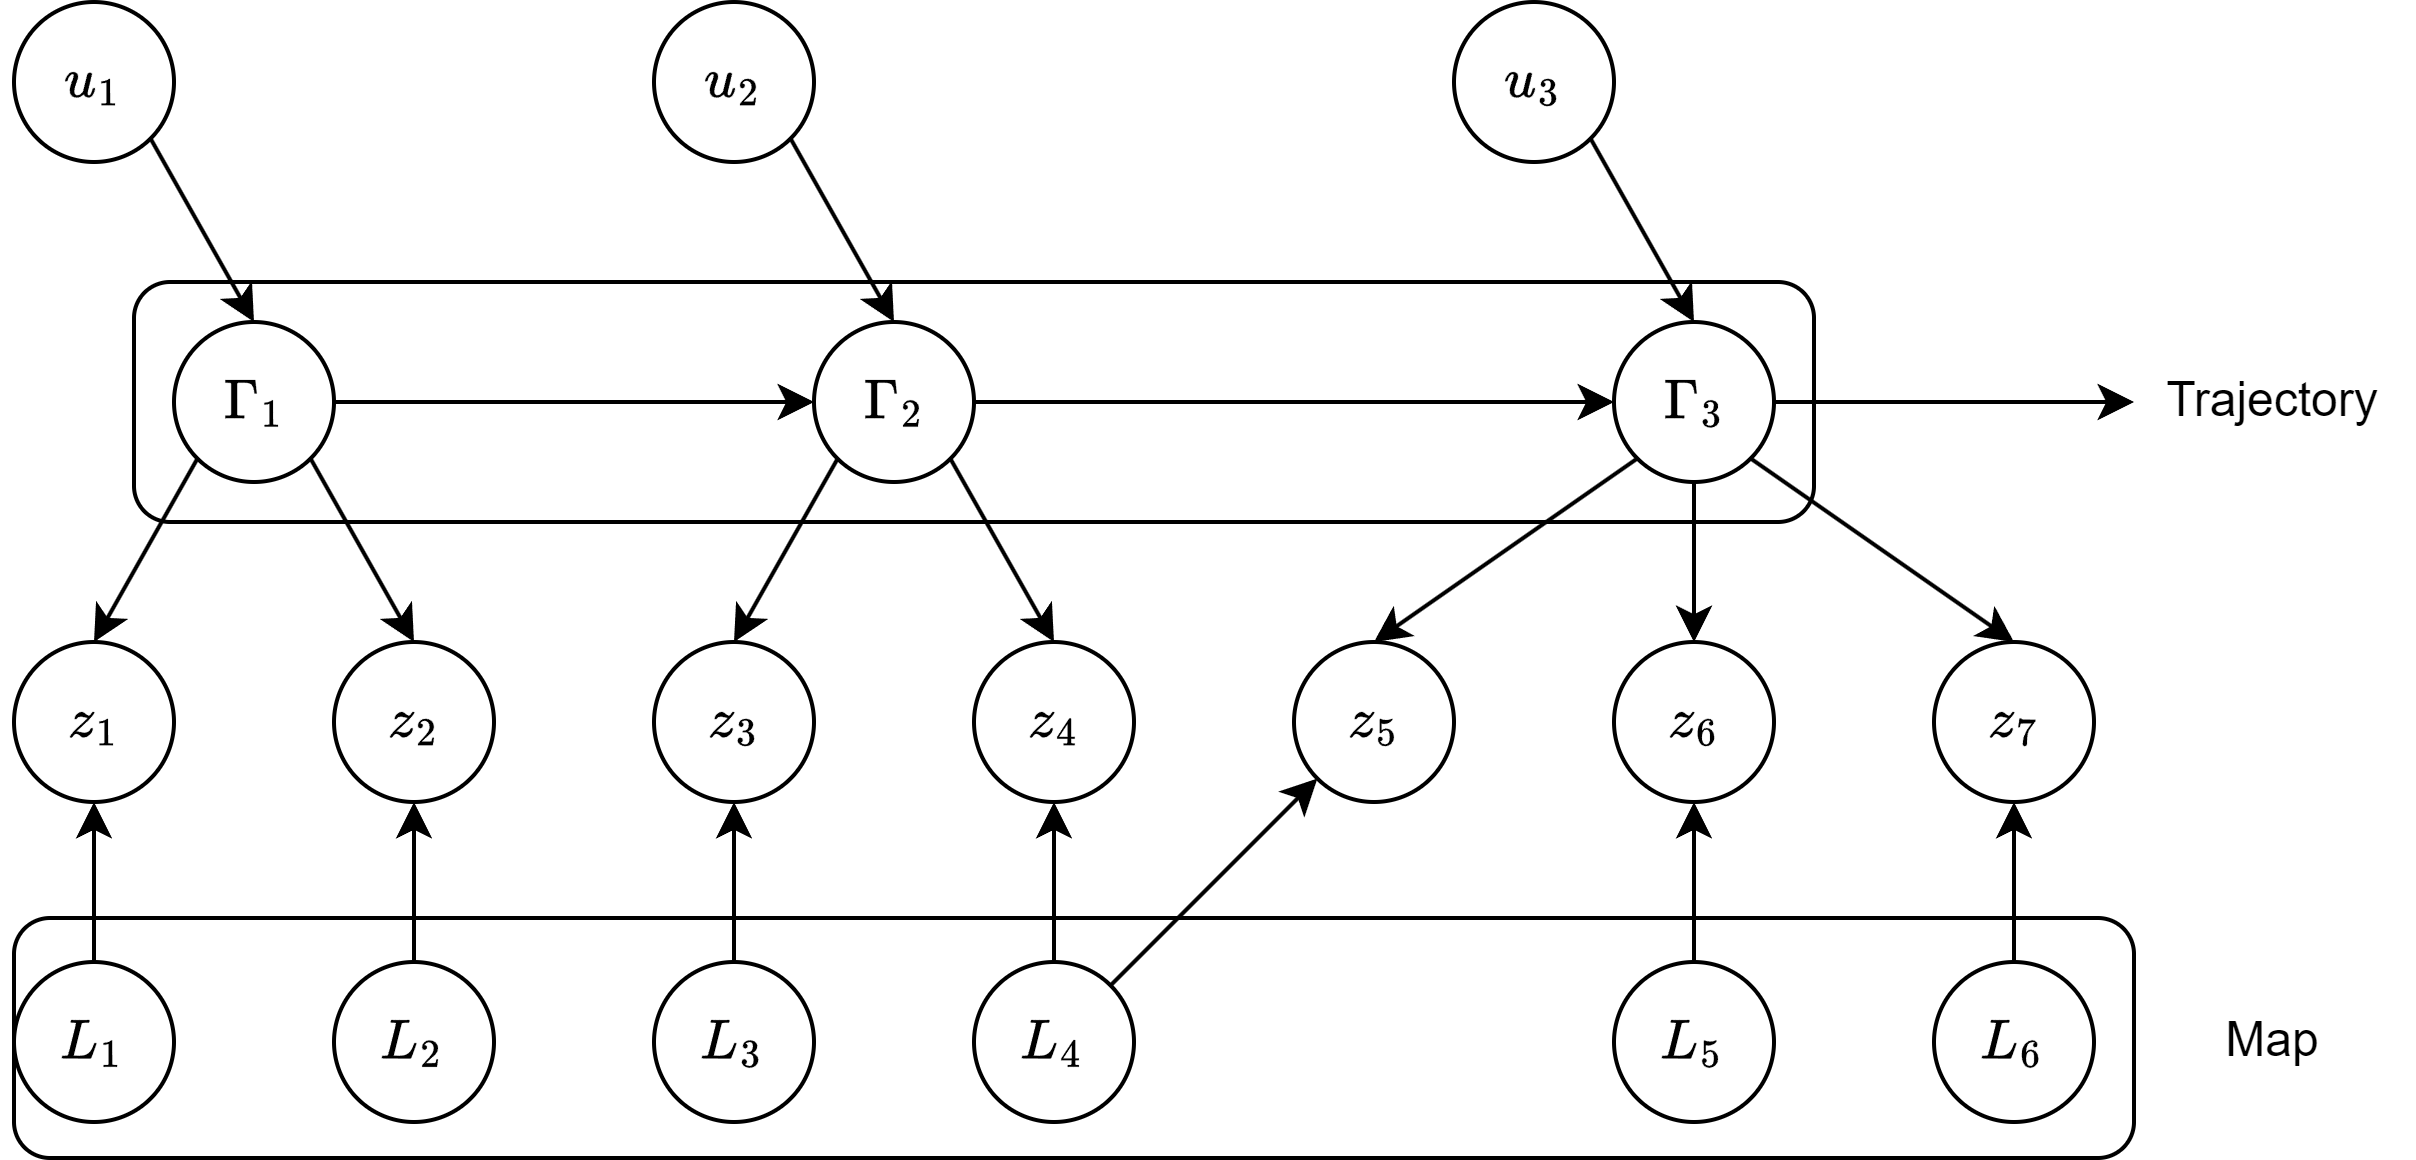
\includegraphics[width=0.75\linewidth]{images/slam.png}
    \caption{Simultaneous Localization and Mapping}
\end{figure}

\paragraph*{Full SLAM}
A full SLAM is achieved when both the map and trajectory are fully computed. 
In this scenario, the probability
\[\Pr(x_{1:t},m|z_{1:t},u_{1:t})\]
is known for each time instant. 
To tackle this problem, FastSLAM can be employed, leveraging a sampled particle filter distribution model.

\paragraph*{Online SLAM}
Online SLAM occurs when we possess the full map but only have knowledge of the current pose. 
In this scenario, we achieve a simultaneous estimate of the most recent pose and map:
\[\Pr(x_t,m|z_{1:t},u_{1:t})=\iint\cdots\int\Pr(x_{1:t},m|z_{1:t},u_{1:t})\,dx_1dx_2\dots dx_{t-1}\]
The integrals are computed sequentially, but if they become overly complex, then opting for full SLAM is preferable. 
For this task, Extended Kalman Filter (EKF) SLAM can be employed, utilizing a linearized Gaussian probability distribution.